
%%% PREAMBLE 
\documentclass[9pt,lineno]{RandlettLab_elife}
\nolinenumbers
\usepackage{lipsum} % Required to insert dummy text
\usepackage{listings}
\usepackage[version=4]{mhchem}
\usepackage{siunitx}
\usepackage{gensymb}
\DeclareSIUnit\Molar{M}
\usepackage{cancel}
\usepackage{xcolor}
\usepackage{textgreek}
\definecolor{codegreen}{rgb}{0,0.6,0}
\definecolor{codegray}{rgb}{0.5,0.5,0.5}
\definecolor{codepurple}{rgb}{0.58,0,0.82}
\definecolor{backcolour}{rgb}{0.96,0.96,0.96}

\lstdefinestyle{mystyle}{
    backgroundcolor=\color{backcolour},   
    commentstyle=\color{codegreen},
    keywordstyle=\color{magenta},
    numberstyle=\tiny\color{codegray},
    stringstyle=\color{codepurple},
    breakatwhitespace=false,         
    breaklines=true,                 
    captionpos=b,                    
    keepspaces=true,                 
    numbers=left,                    
    numbersep=5pt,                  
    showspaces=false,                
    showstringspaces=false,
    showtabs=false,                  
    tabsize=2
}

\lstset{style=mystyle}

%%%%%%%%%%%%%%%%%%%%%%%%%%%%%%%%%%%%%%%%%%%%%%%%%%%%%%%%%%%%
%%% ARTICLE SETUP
%%%%%%%%%%%%%%%%%%%%%%%%%%%%%%%%%%%%%%%%%%%%%%%%%%%%%%%%%%%%
\title{Estradiol increases visual habituation learning independently of the canonical estrogen receptors}

\author[ !,1,2] 
{Andrew Hsiao}

\author[ !,1] 
{Isabelle Darvaux-Hubert}

\author[ 1,3] 
{Dominique Hicks}

\author[ 1,2] 
{Emilie Joux}

\author[ 1,2]
{Sarah De Freitas}

\author[ 1,2]
{Emeline Dracos}

\author[ 1,2]
{Jeanne Litze}

\author[1] 
{Julien Perrichet}

\author[ *,1] 
{Dominique Baas}

\author[ *,@,1] 
{Owen Randlett}


\affil[1]{
Laboratoire MeLiS, Université Claude Bernard Lyon 1 - CNRS UMR5284 - Inserm U1314, Institut NeuroMyoGène, Faculté de Médecine et de Pharmacie, 8 avenue Rockefeller, 69008 Lyon, France
}

\affil[2]{
International Master in Life Sciences, Université Claude Bernard Lyon 1, France
}

\affil[3]{
Master of Biology Program, École normale supérieure de Lyon, France
}

\affil[!]{equal contribution}

\affil[*]{equal contribution}


\affil[@]{correspondence: \href{mailto:owen.randlett@univ-lyon1.fr}{owen.randlett@univ-lyon1.fr}}

%%%%%%%%%%%%%%%%%%%%%%%%%%%%%%%%%%%%%%%%%%%%%%%%%%%%%%%%%%%%
%%% ARTICLE START
%%%%%%%%%%%%%%%%%%%%%%%%%%%%%%%%%%%%%%%%%%%%%%%%%%%%%%%%%%%%

\begin{document}

\maketitle
\begin{abstract}

Habituating to the constant stimuli in the environment is a critical adaptive learning process conserved across species. 
We use the larval zebrafish visual response to sudden darkness as a model for studying habituation learning, where zebrafish reduce their responses to repeated stimulations. 
In this paradigm, treatment with Estradiol strongly increases learning rate, resulting in reduced responses. 
In an attempt to identify the receptor(s) mediating these effects we used established mutant lines for the known estrogen receptors (\emph{esr1}, \emph{esr2a}, \emph{esr2b}, \emph{gper1}). 
Our experiments failed to identify a receptor required for the effects of Estradiol on habituation learning. 
Surprisingly, \emph{esr1}, \emph{esr2a}, and \emph{gper1} mutants showed weak but consistent increases in habituation relative to sibling controls, indicating that activation of these receptors may have paradoxical inhibitory effects on habituation learning. 
These experiments confirm that estradiol is a potent modulator of learning processes in the vertebrate brain, but in the context of visual habituation learning in larval zebrafish, these effects do not occur via the classical estrogen receptor-mediated signaling pathways, which instead act in competition to subtly inhibit habituation learning. 
Therefore, our data indicate that the positive effects of estradiol on habituation learning occur via an as-yet unidentified receptor, or via allosteric modulation of a parallel signaling pathway.

\end{abstract}

\section{Introduction}

A primary task of the brain is to learn from ongoing experiences and adjust behavior accordingly. 
This often involves sharpening attention and behavioural resources toward salient cues while tuning out irrelevant background stimuli. 
For instance, it may be critical to recognize the alarm calls of a nearby animal, whereas continually registering a steady hum from distant traffic is far less important. 
The capacity to reduce responses to repetitive, non-essential stimuli is known as habituation, a phenomenon widely considered one of the simplest forms of learning and memory \citep{Rankin2009-no}. 

We have been studying a paradigm for long-term habituation where larval zebrafish reduce their responsiveness to sudden pulses of whole-field darkness, or dark flashes (DFs) \citep{wolman_chemical_2011, Randlett2019-fj, Lamire2023-he}. 
In this analysis, we emphasize long-term habituation as a practical model for examining the fundamental processes that shape neural circuit plasticity.
We recently reported that multiple hormonal signaling pathways show strong modulation of habituation learning performance, including Melatonin, progesterone, and estrogen \citep{Lamire2023-he}. 
The ability of these signaling pathways to modulate learning is consistent with previous results in other systems and paradigms \citep{Nilsson2002-as, Naderi2020-ot, Dillon2013-rk, Rawashdeh2007-bw, Jilg2019-oy, El-Sherif2003-vt, Barros2015-jm}, and may be an important mechanism to shift learning and memory performance or strategies based on biological rhythms or external fluctuations like seasons, weather or the day/night cycle.

In this project we have focused on the Estrogen Receptors (ERs), since we identified multiple estradiol analogs (ethinyl estradiol, estradiol valerate, and hexestrol), which strongly increased habituation learning when applied at 5-10\textmu M doses in the water \citep{Lamire2023-he}.
Estradiol is the most potent and biologically active form of estrogen, and is used in a variety of clinical contexts including contraception, hormone replacement therapy and gender-affirming therapy.  



Estrogen signaling in learning and memory, any data about receptors. 

In this project we aimed to identify the relevant estrogen receptor mediating the effects of estradiol analogs on habituation learning by undertaking a classical analysis of genetic knockout alleles. 
Not only did we fail to identify a mutant (or combination of mutants) that lead to estradiol insensitivity, leading us to conclude that these receptors act to inhibit habituation learning, rather than mediating the habituation-promoting effects of Estradiols in the zebrafish brain. 
estrogne receptor mutants that show increased sensitivity to estradiol in the habituation paradigm. 


%\newpage
\section{Materials and Methods}

\subsection{Animal Ethics Statement}

Adult zebrafish used to generate larvae were housed in accordance with PRCI facility approved by the animal welfare committee (comité d’éthique en expérimentation animale de la Région Rhône-Alpes: CECCAPP, Agreement \# C693870602). 
Behaviour experiments were performed at the 5dpf stage, and are thus not subject to ethical review, but these procedures do not harm the larvae. 

\subsection{Animals}

All experiments were performed on larval zebrafish at 5 days post fertilization (dpf), raised at a density of $\approx$1 larvae/mL of E3 media supplemented with 0.02\% HEPES pH 7.2. 
Larvae were raised in a 14:10h light/dark cycle at 28-29\degree{}C. 
Adult zebrafish were housed, cared for, and bred at the Lyon PRECI zebrafish facility. 
Mutant lines were obtained from D. Gorelick's lab, and were of the following alleles: 

\emph{esr1\textsuperscript{uab118}} is a 4bp deletion (ZDB-ALT-180420-2), yielding a predicted null frameshift/stop mutation, confirmed by a lack of estradiol responsiveness in the heart as assayed by \emph{Tg(5xERE:GFP)\textsuperscript{c262}} expression \citep{Romano2017-ep}. 

\emph{esr2a\textsuperscript{uab134}} is a 2bp deletion (ZDB-ALT-180420-3), yielding a predicted null frameshift/stop mutation \citep{Romano2017-ep}

\emph{esr2b\textsuperscript{uab127}} is a 4bp deletion (ZDB-ALT-180420-4), yielding a predicted null frameshift/stop mutation, confirmed by a lack of estradiol responsiveness in the liver as assayed by \emph{Tg(5xERE:GFP)\textsuperscript{c262}} expression \citep{Romano2017-ep}. 

\emph{gper1\textsuperscript{uab102}} is a 133bp deletion (ZDB-ALT-180420-1), yielding a predicted null frameshift/stop mutation, confirmed by a lack of estradiol responsiveness in heart beating rate in maternal-zygotic mutants \citep{Romano2017-ep}.

\subsection{Genotyping}

% Esr1 is the uab118 (https://zfin.org/ZDB-ALT-180420-2) line from Gorelick Lab . 
% Mutation is a 4 bp  (CGGC) deletion on chromosome 20 obtained after CRISPR, 
% resulting on a premature stop codon.
\emph{esr1\textsuperscript{uab118}} was genotyped by PCR using the forward/reverse primer pair:
\\ \mbox{GCTGGTCACCTTGAATGCTT/TGAGATGTGAGAGATGACTAGGA} with a T\textsubscript{M} of 58°C yielding a 381 bp PCR product that was digested with the restriction enzyme ApeKI. 
The mutant product is not digested, and the wild type has two bands at 177 and 204 bp.

\emph{esr2a\textsuperscript{uab134}} was genotypes by PCR using the forward/reverse primer pair:
\\ \mbox{CTTCAGCTGCAGGAAGTGGA/AAAGTCGGGCTTAGCGACTG} with a T\textsubscript{M} of 58°C yielding a 236 bp PCR product that was digested with the restriction enzyme MboI.
The mutant product is not digested, and the wild type has two bands at 180 and 56 bp 

\emph{esr2b\textsuperscript{uab127}} was genotypes by PCR using the forward/reverse primer pair:
\\ \mbox{TGGGCCTGAGATGCAGTAGT/GTGTGTGTCTTGGCCTCCTC} with a T\textsubscript{M} of 60°C yielding a 431 bp PCR product that was digested with the restriction enzyme MbiI.
The mutant product is digested into two bands of 150 and 281 bp and the wild type into 3 bands of 78, 150 and 198 bp. 

\emph{gper1\textsuperscript{uab102}} was genotypes by PCR using the forward/reverse primer pair:
\\ \mbox{ATGGAGGAGCAGACTACCAATGTG/CCATCCAGATGAGGCTGCAA} with a T\textsubscript{M} of 60°C yielding a mutant product of 372bp and a wild type product of 505 bp.


\subsection{Pharmacology}

\textbeta-Estradiol (Sigma E2758, here referred to as "estradiol") was dissolved in dimethyl sulfoxide (DMSO) and stored at -20\degree C. 
Larvae were treated with estradiol immediately before the behavioural assay by pipetting 10-30uL of 10x solution directly into the behavioural wells, always with a final concentration of 0.1\% DMSO in E3.

\subsection{Habituation behaviour testing}

asdfadffffffffffffffffffffasdfasdfasfd

\subsection{Data analysis}

Data was analzed in python using custom written analysis scripts, available on \href{https://github.com/owenrandlett/2025\_HabEstrogen}{github}. 


\newpage
\section{Results and Discussion}

\subsection{Estradiol increases habituation learning}


\begin{figure}
\begin{fullwidth}
\begin{center}
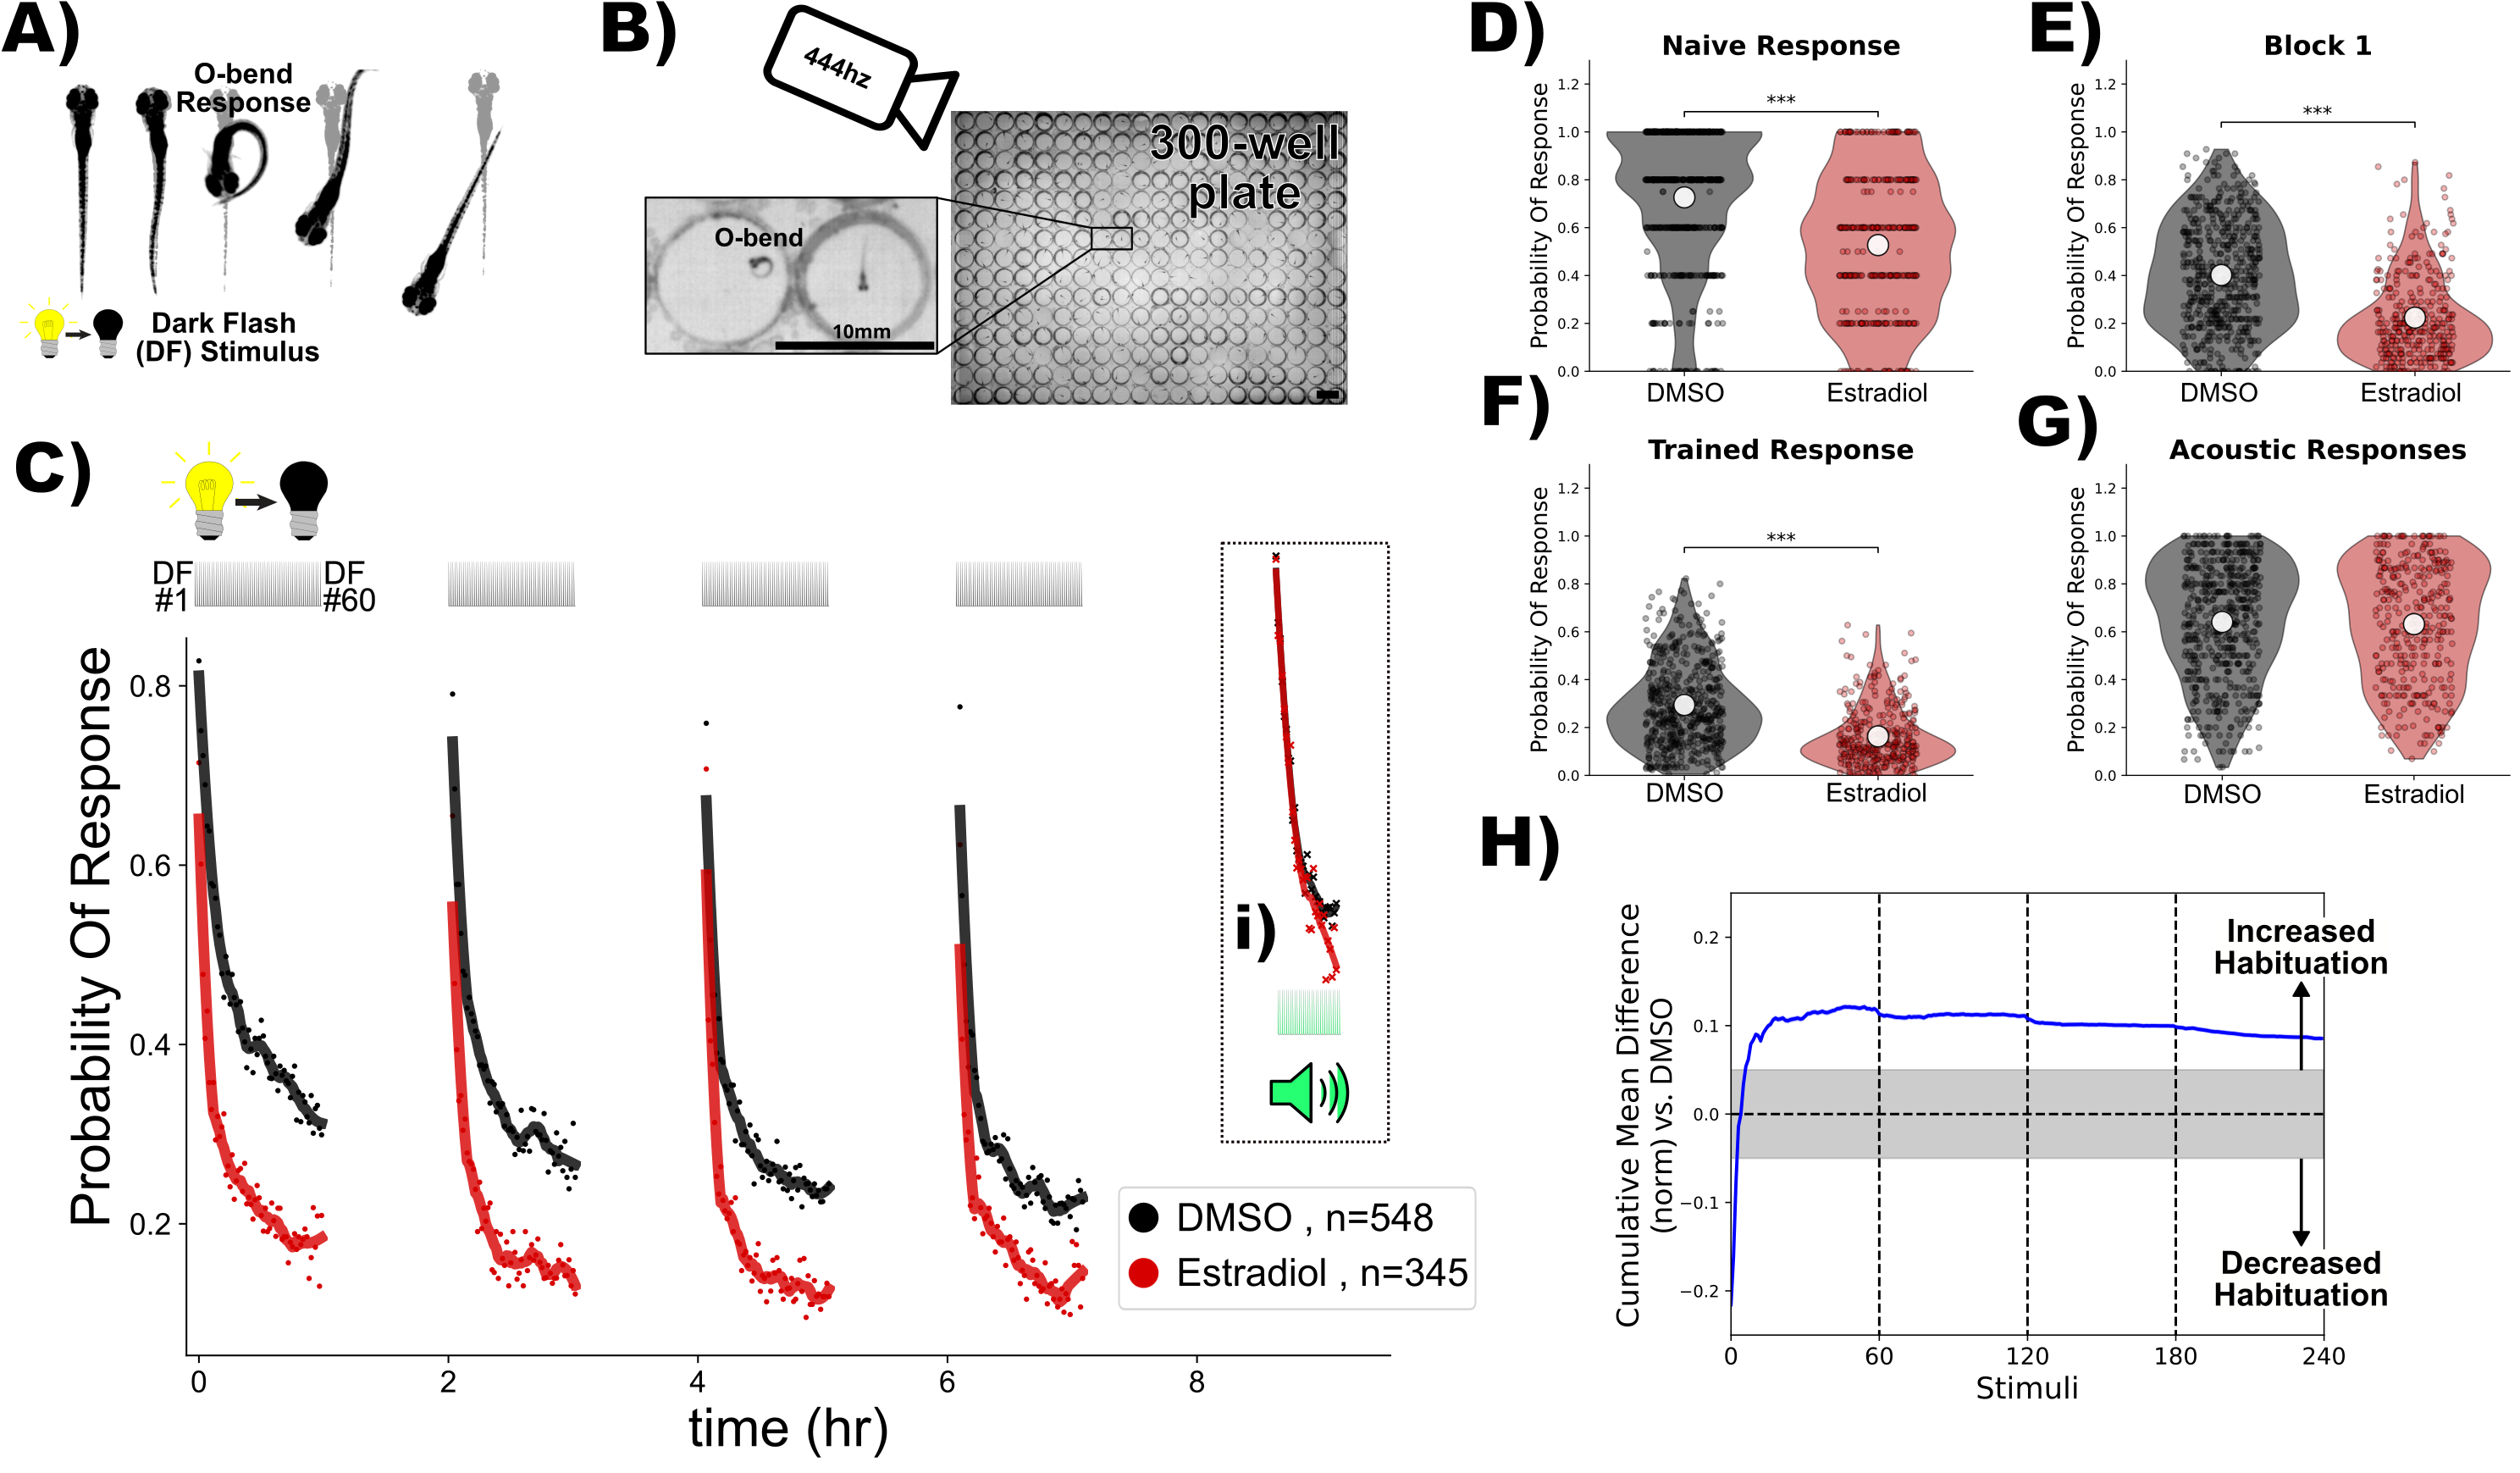
\includegraphics[width=0.75\linewidth]{figures/EstradiolEffect.png}
\caption{\textbf{Estradiol increases habituation learning.}
\\ \textbf{A)} In response to a dark flash (DF), larval zebrafish perform a large turning maneuver termed an O-bend response.
\\ \textbf{B)} High-throughput setup for recording and quantify O-bend responsiveness using a high-speed camera recording at 444hz observing larvae in 300-well plates.
\\ \textbf{C)} Treatment with estradiol (red) results in more rapid and profound decreases in the probability of response to DF stimuli during habituation training relative to DMSO vehicle controls (black). DF stimuli are delivered at 1-minute intervals, in 4 blocks of 60 stimuli, separated by 1hr of rest (from 0:00-7:00). 1.5 hours later a block of 30 acoustic stimuli are delivered at 1-minute intervals (\textbf{i}). Each dot is the probability of response to one DF. Lines are smoothed in time with a Savitzky–Golay filter (window = 15 stimuli, order = 2). 
\\ \textbf{D-G)} Distributions responsiveness for different epochs of the experiment. Each dot is the per-fish average of the epoch. Statistical significance was calculated using Mann-Whitney U test, *** = p < 0.001.  \textbf{D)} the naive response to the first 5 DF stimuli; \textbf{E)} the mean response to the remaining DF stimuli in the Block 1 (DFs 6:60); \textbf{F)} the trained response to the last 45 DFs in all four training blocks (DFs 16:60,76:120,136:180,196:240); \textbf{G)} the 30 acoustic stimuli delivered with a tap from a solenoid on the 300-well plate platform. 
\\ \textbf{H)} Cumulative mean difference plot quantifying relative habituation performance after estradiol treatment. These plots display the cumulative average differences in the mean response across larvae of the treatment group (estradiol) relative to the control group (DMSO). Difference from 0 reflect a divergence in the change in responsivness across the 240 DF stimuli in the 4 training blocks, with positive values reflecting increased habituation. The widths of the line is a bootstrapped 99.5\% confidence intervals. The gray boxed region reflects the expected non-significant effect size \citep{Randlett2019-fj}.
\\ Treatment groups are: Estradiol = 10\textmu M estradiol treatment (n = 345 fish); DMSO = 0.1\% DMSO vehicle controls (n = 548 fish)
}

\label{fig:1}

\end{center}
\end{fullwidth}
\end{figure}


In response to a sudden global dimming event, which we refer to as a dark flash (DF), larval zebrafish execute an "O-bend" maneuver, characterized by a deep "O"-shaped bend and a high-amplitude turn \citep{Burgess2007}. 
Habituation learning manifests as a progressive reduction in response to repeated stimuli, and this learning can be retained for seconds/minutes or hours/days for short- and long-term habituation, respectively \citep{Rankin2009-no}. 
We use high-speed cameras, machine-vision analysis, and 300-well plates to quantify habituation across large populations of larvae to identify molecular/genetic mechanisms of long-term habituation({\autoref{fig:1}A,B, \citealp{Randlett2019-fj,Lamire2023-he}). 
When stimulated with DFs repeated at 1-minute intervals in repeated blocks of 60 stimuli, larval zebrafish exhibit long-term habituation, reducing not only the probability of executing a response, but also modulating the latency and other kinematic aspects of the response \citep{Randlett2019-fj}.  

Our previous small-molecule screening experiments identified multiple synthetic Estrogen Receptor agonists as positive modulators of dark-flash habituation learning, including ethinyl estradiol, estradiol valerate, and hexestrol  \citep{Lamire2023-he}. 
The major effect we observed was a stronger decrease in the probability of executing a O-bend response during the training/learning blocks. 
We have confirmed and extended these results using \textbeta-Estradiol (estradiol), which is the major natural estrogen in humans. 
An acute dose of 10\textmu M estradiol potently increases habituation learning, which is observable when the response probability of the population of estradiol-treated larvae is compared with DMSO-treated vehicle controls across stimuli (\autoref{fig:1}C-H).
Consistent with our previous experiments \citep{Lamire2023-he}, there is a modest reduction in the initial responsiveness of the estradiol-treated larvae to the first DF stimulus (\autoref{fig:1}D), but the major effect is observed during the training phase (\autoref{fig:1}C,E,F), as is revealed by the consistent positive deviation in the cumulative mean difference plot (\autoref{fig:1}H, \citealp{Randlett2019-fj}).
Importantly, the responsiveness of the larvae to acoustic stimuli delivered after the DF training is indistinguishable from controls (\autoref{fig:1}Ci, G), indicating that estradiol does not affect global arousal levels but rather has specific effects on habituation learning. 


\subsection{Membrane-initiated estradiol signaling via Gper1 does not increase habituation learning}

\begin{figure}
\begin{fullwidth}
\begin{center}
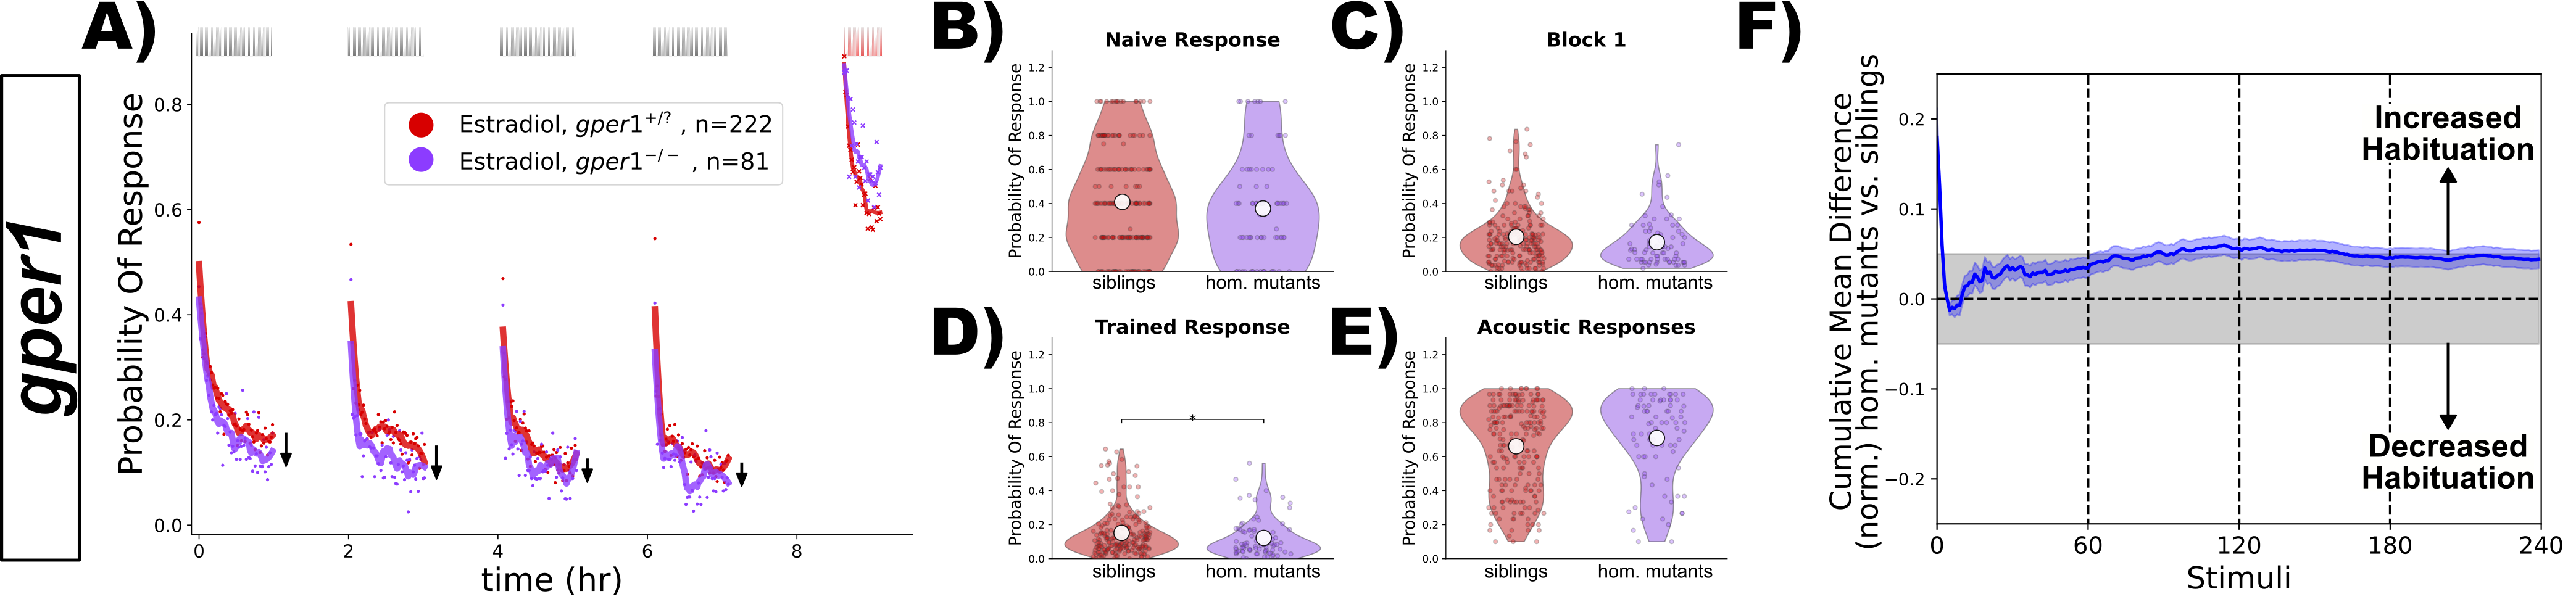
\includegraphics[width=0.95\linewidth]{figures/gper1Mutants.png}
\caption{\textbf{\emph{gper1} mutants do not show habituation deficits after treatment with estradiol.}
\\ \textbf{A)} Homozygous \emph{gper1\textsuperscript{(-/-)}} mutants do not show impaired habituation relative to sibling controls (\emph{gper1\textsuperscript{(+/-)}} and \emph{gper1\textsuperscript{(+/+)}}). Rather, there is a slight suppression of responsiveness in the mutant group, indicating weakly increased habituation. 
\\ \textbf{B-E)} No significant differences are observed in the responsiveness distributions for the naive response to the first 5 DF stimuli (\textbf{B}), during the first training block (\textbf{C}), or the acoustic response (\textbf{E}), while a subtle but statistically significant decrease in responsiveness is observed in the trained response (\textbf{D}). Statistical significance was calculated using Mann-Whitney U test, * = p < 0.05.
\\ \textbf{F)} Cumulative mean difference plot quantifying relative habituation performance in  after estradiol treatment, consistent with slightly increased habituation rate in mutant larvae. 
}
\label{fig:2}

\end{center}
\end{fullwidth}
\end{figure}

The effects of estradiol we have observed occur very rapidly -- larvae are only pretreated with estradiol for $\approx$25min-1hr before the first DF, as this is the time necessary to set the apparatus and begin the experiment.
Since classical nuclear hormone receptors (like the Esr1 and Esr2) exert their effects via transcriptional adaptation, this necessitates a delay in signaling response. 
Therefore, we hypothesized that membrane initiated signaling through Gper1 was the more likely mechanism. 
To test this we obtained and tested the presumed null frameshift/early stop allele \emph{gper1\textsuperscript{uab102}}, which was previously shown to be insensitive to estradiol for heart-rate modulation \citep{Romano2017-ep}. 

To test if \emph{gper1} is required for the effects of estradiol on habituation we generated larvae from \emph{gper1\textsuperscript{uab102}} heterozygous or homo/hererozygous crosses to generate clutches of larvae of mixed genotypes. Larvae were treated with estradiol during habituation, and were subsequently genotyped. We reasoned that if \emph{gper1} is required for the effect of estradiol on habituation, mutants would habituate significantly less than controls. Contrary to this hypothesis, we found that \emph{gper1} mutants showed no deficits in habituation (\autoref{fig:2}). Remarkably, rather than observing the anticipated inhibition of habituation, \emph{gper1} mutants appeared to habituate slightly more, with the responsiveness trendline running slightly but consistently below the sibling controls (\autoref{fig:2}A). This is further supported by a weak but statistically significant decrease in the responsiveness of the larvae during the training period (\autoref{fig:2}D), and a trend towards positive values in the Cumulative Mean DIfference plot (\autoref{fig:2}F). 

From these experiments we conclude that: 
\\ \textbf{1)} Gper1 does not mediate the positive effects of estradiol on habituation learning, and therefore these effects are mediated by a different receptor. 
\\ \textbf{2)} Gper1 appears to have a paradoxical inhibitory effect on habituation learning, although this effect size is relatively minor and does not rise substantially above biological noise levels. 
\\ \textbf{3)} The observed paradoxical inhibitory effect confirms that these mutants do have a phenotype in our assay, despite it not being of the predicted sign. This provides compelling evidence that our negative results do not simply result from an issue or mischaracterization of this predicted null-allele \citep{Romano2017-ep}.  

\subsection{Nuclear-mediated estradiol signaling via Esr1, Esr2a or Esr2b does not increase habituation learning}

\begin{figure}
\begin{fullwidth}
\begin{center}
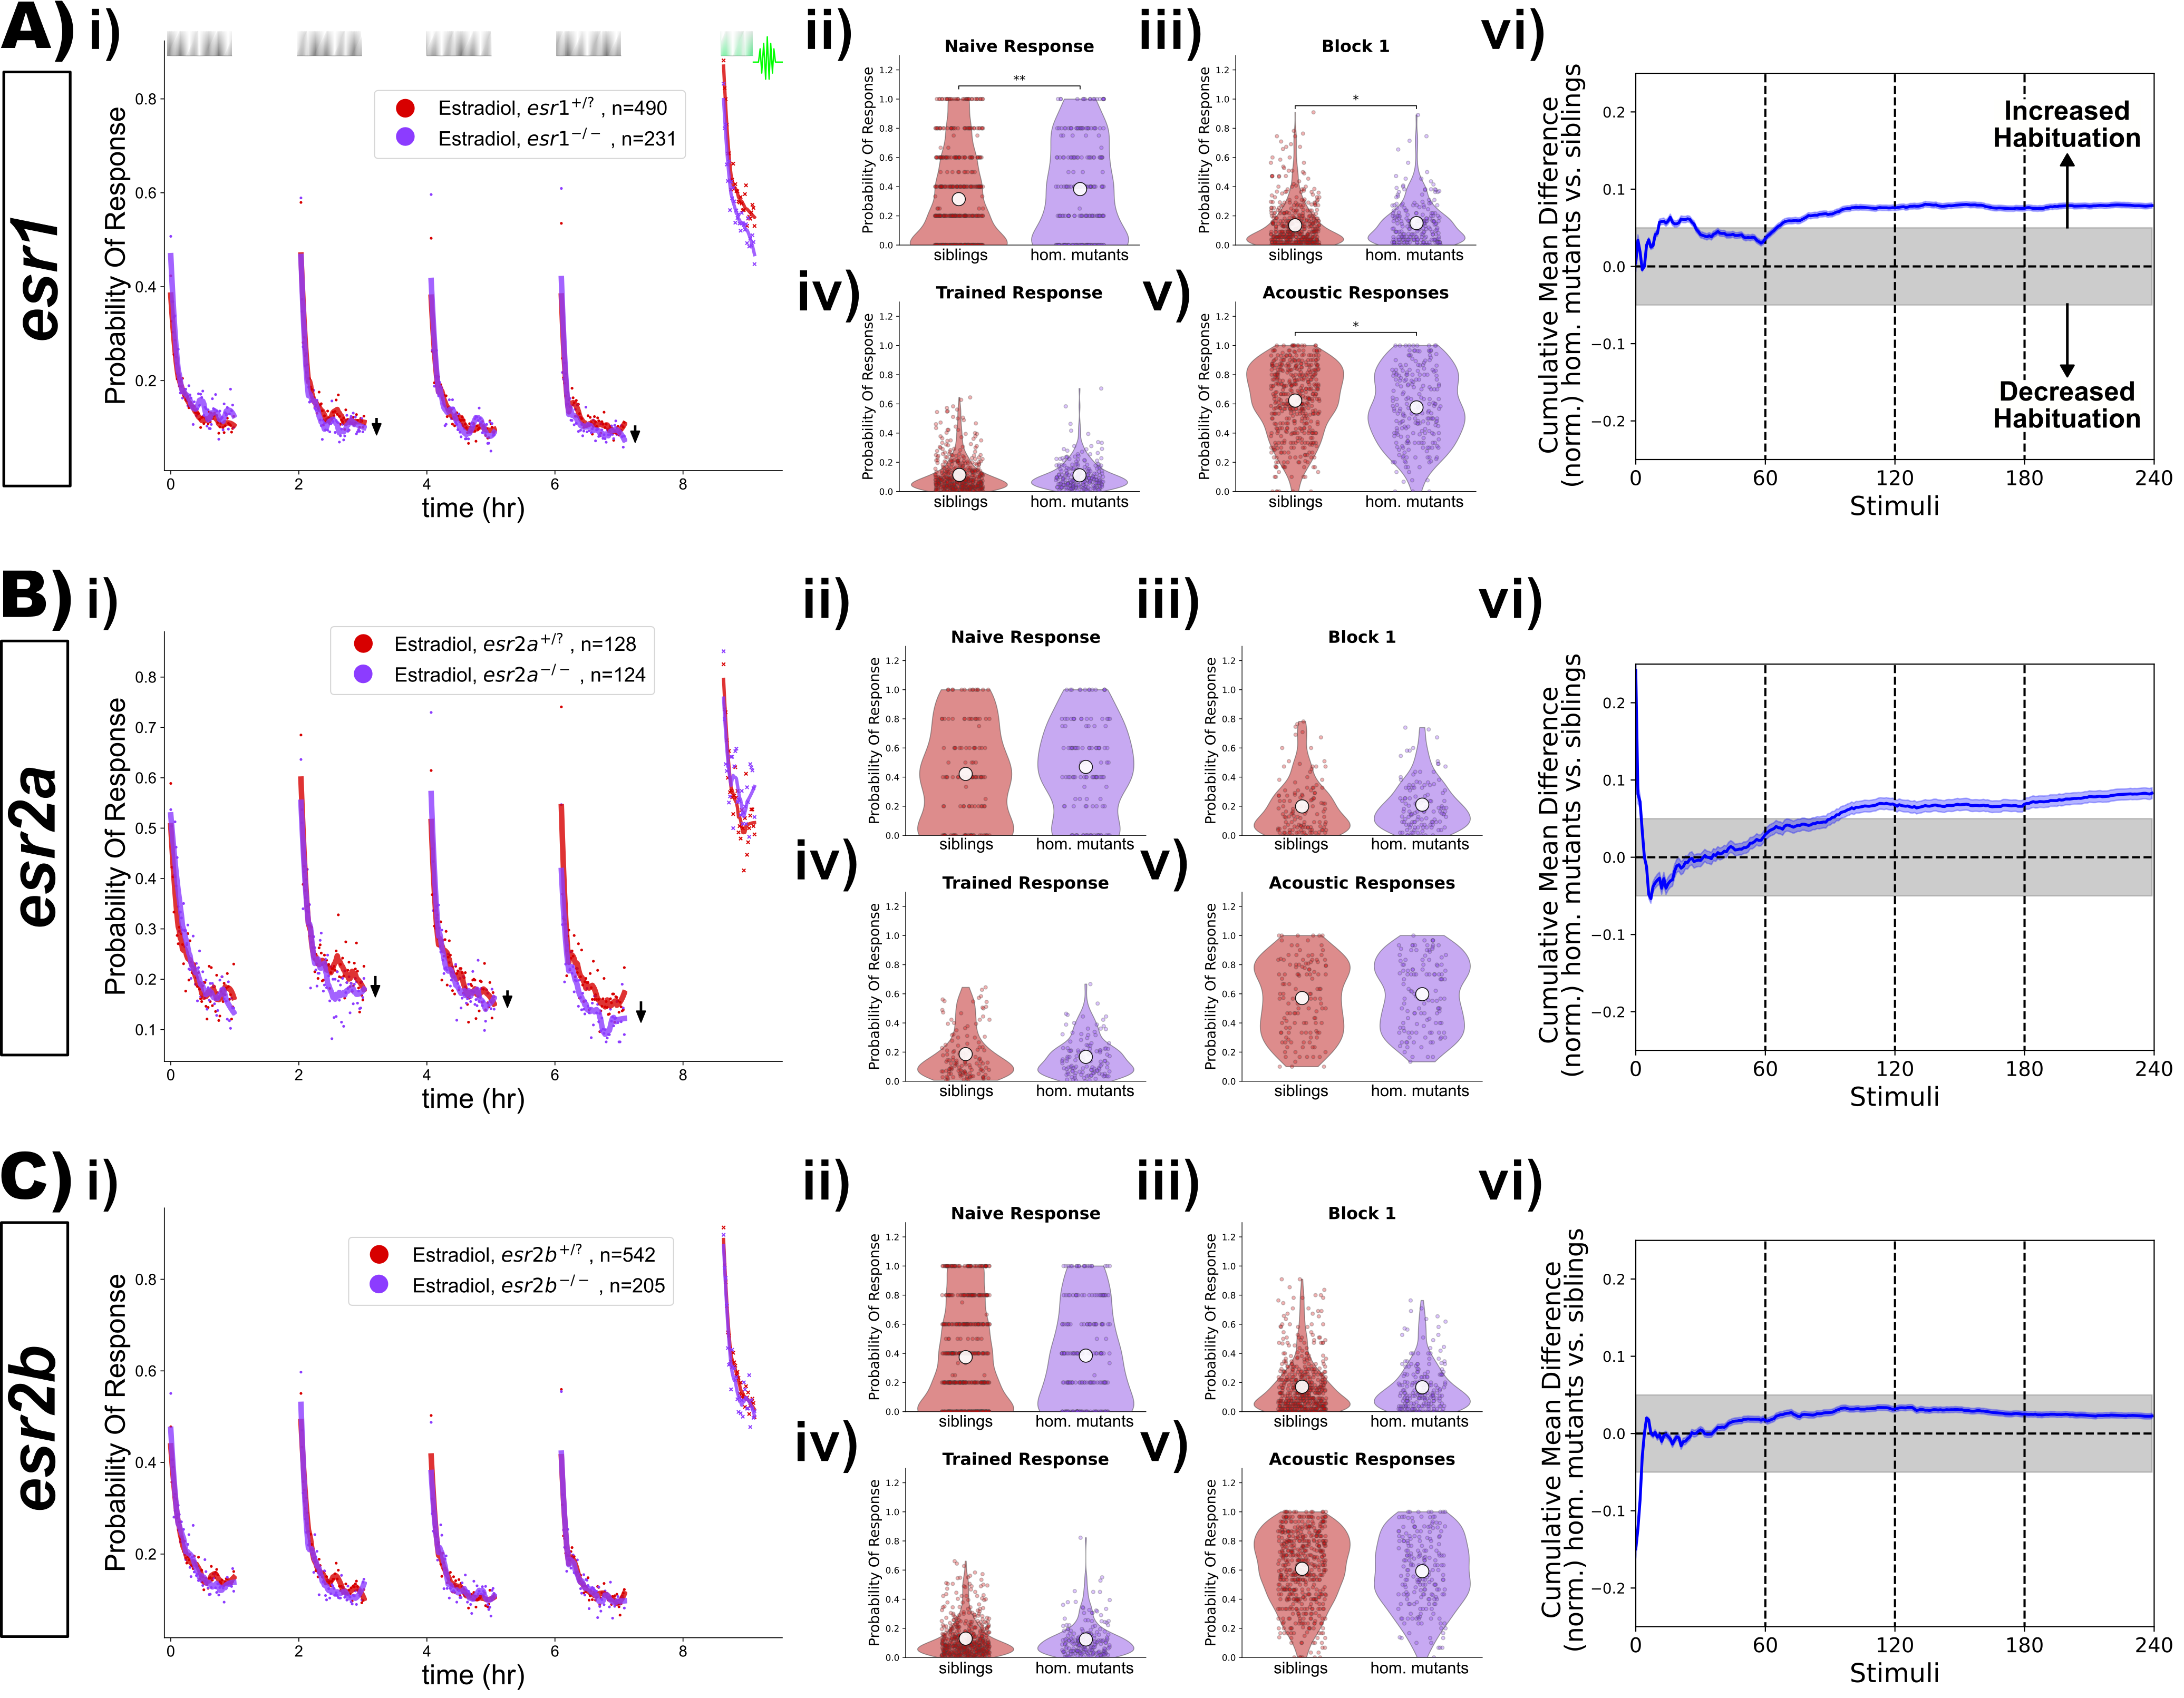
\includegraphics[width=0.95\linewidth]{figures/NuclearSingleMutants.png}
\caption{\textbf{\emph{esr1}, \emph{esr2a} and \emph{esr2a} mutants do not show habituation deficits after treatment with estradiol.}
\\ \textbf{A)} Homozygous \emph{esr1\textsuperscript{(-/-)}} mutants do not show impaired habituation relative to sibling controls (\emph{esr1\textsuperscript{(+/-)}} and \emph{esr1\textsuperscript{(+/+)}}). 
\\ \textbf{B)} Homozygous \emph{esr2a\textsuperscript{(-/-)}} mutants do not show impaired habituation relative to sibling controls (\emph{esr2a\textsuperscript{(+/-)}} and \emph{esr2a\textsuperscript{(+/+)}}).
\\ \textbf{C)} Homozygous \emph{esr2b\textsuperscript{(-/-)}} mutants do not show impaired habituation relative to sibling controls (\emph{esr2b\textsuperscript{(+/-)}} and \emph{esr2b\textsuperscript{(+/+)}}). 
}
\label{fig:3}

\end{center}
\end{fullwidth}
\end{figure}

Since we found the \emph{gper} was unnecessary for the positive effects of estradiol on habituation learning, we next focused on the three nuclear receptors in the zebrafish genome: \emph{esr1}, \emph{esr2a} and \emph{esr2a}. Using the same strategy as for \emph{gper}, we analyzed previously established and presumed null mutants (\emph{esr2a\textsuperscript{uab134}}, \emph{esr2a\textsuperscript{uab134}}, and \emph{esr2b\textsuperscript{uab127}}), looking for a mutant with habituation deficits after estradiol treatment. However, we again failed to identify any decreases in habituatuin (\autoref{fig:3}), and to our surpise we again found that both \emph{esr1} and \emph{esr2a} mutants showed sublte \textbf{increases} in habituation (\autoref{fig:3}Avi,Bvi), similar in magnitude to what we had seen for \emph{gper1} mutants (\autoref{fig:2}F). 

\begin{figure}
\begin{fullwidth}
\begin{center}
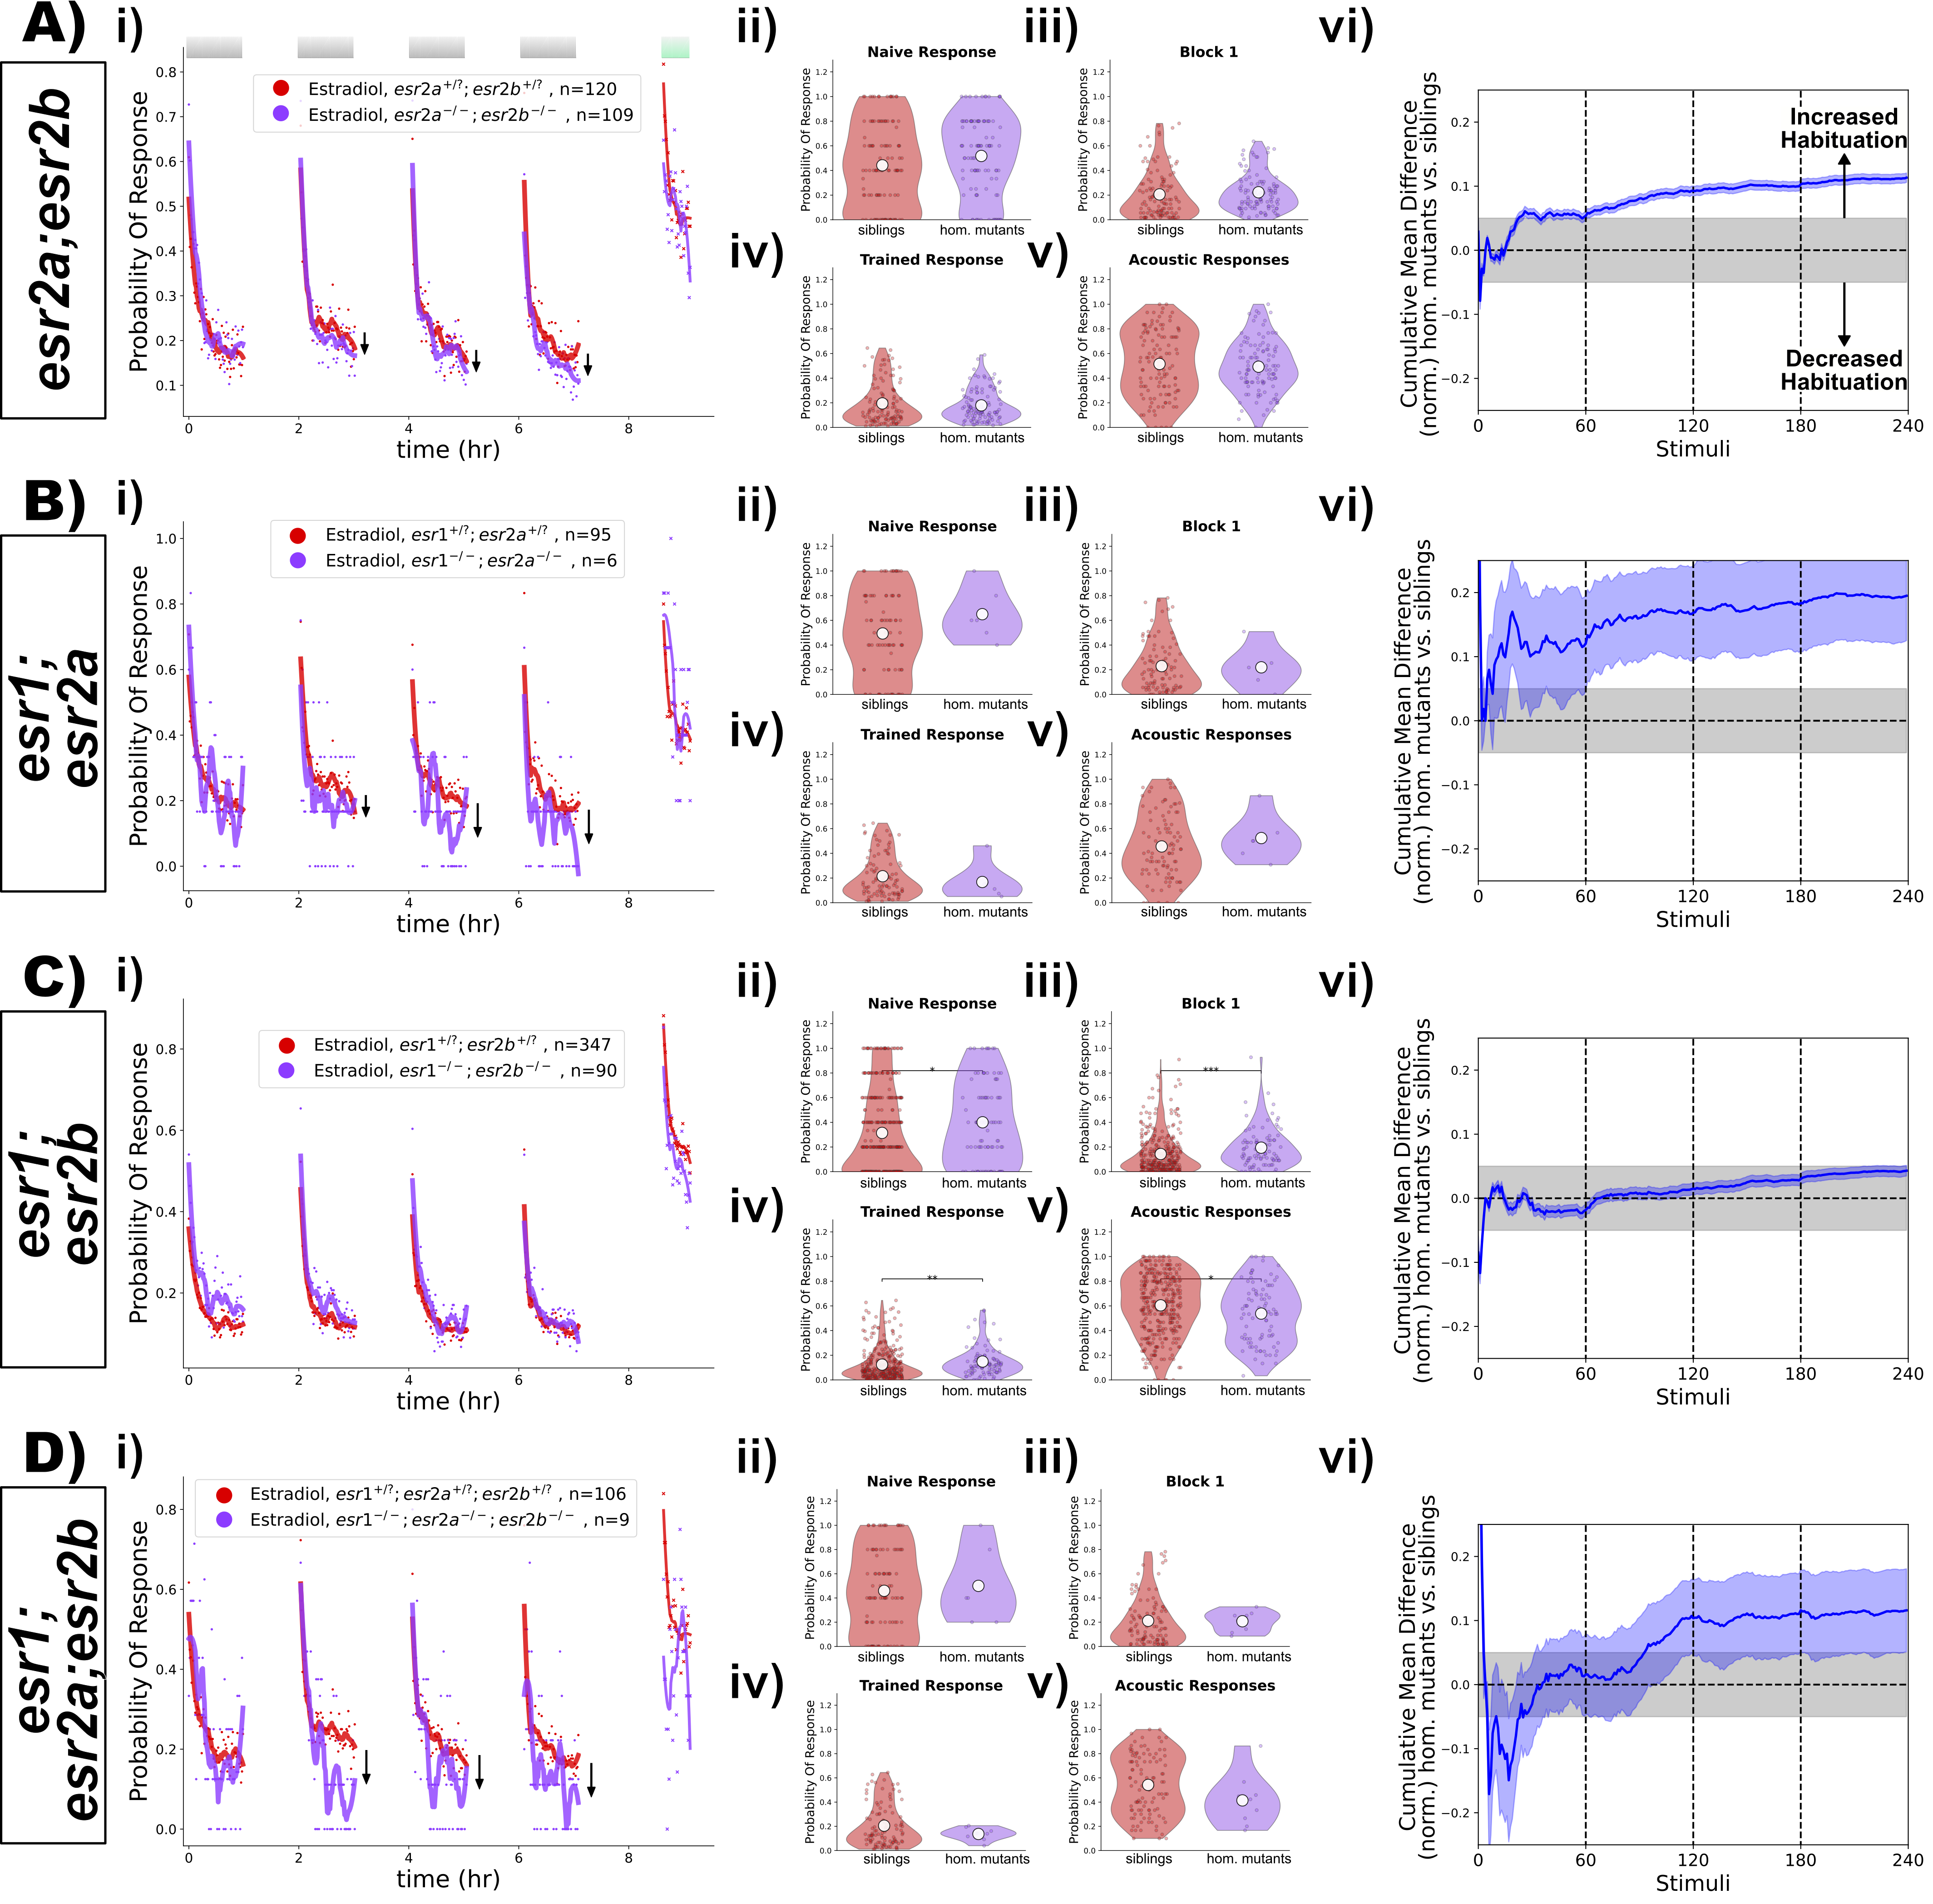
\includegraphics[width=0.95\linewidth]{figures/NuclearDoubleAndTripleMutants.png}
\caption{ \textbf{Double and triple mutant combinations of \emph{esr1}, \emph{esr2a} and \emph{esr2a} do not show habituation deficits after treatment with estradiol.}
\\ \textbf{A)} Homozygous \emph{esr1\textsuperscript{(-/-)}} mutants do not show impaired habituation relative to sibling het/wt controls. 
}
\label{fig:4}

\end{center}
\end{fullwidth}
\end{figure}

\subsection{Membrane-initiated and nuclear-mediated signaling are simultaneously dispensible for estradiol-induced enhancements in habituation learning}

\begin{figure}
\begin{fullwidth}
\begin{center}
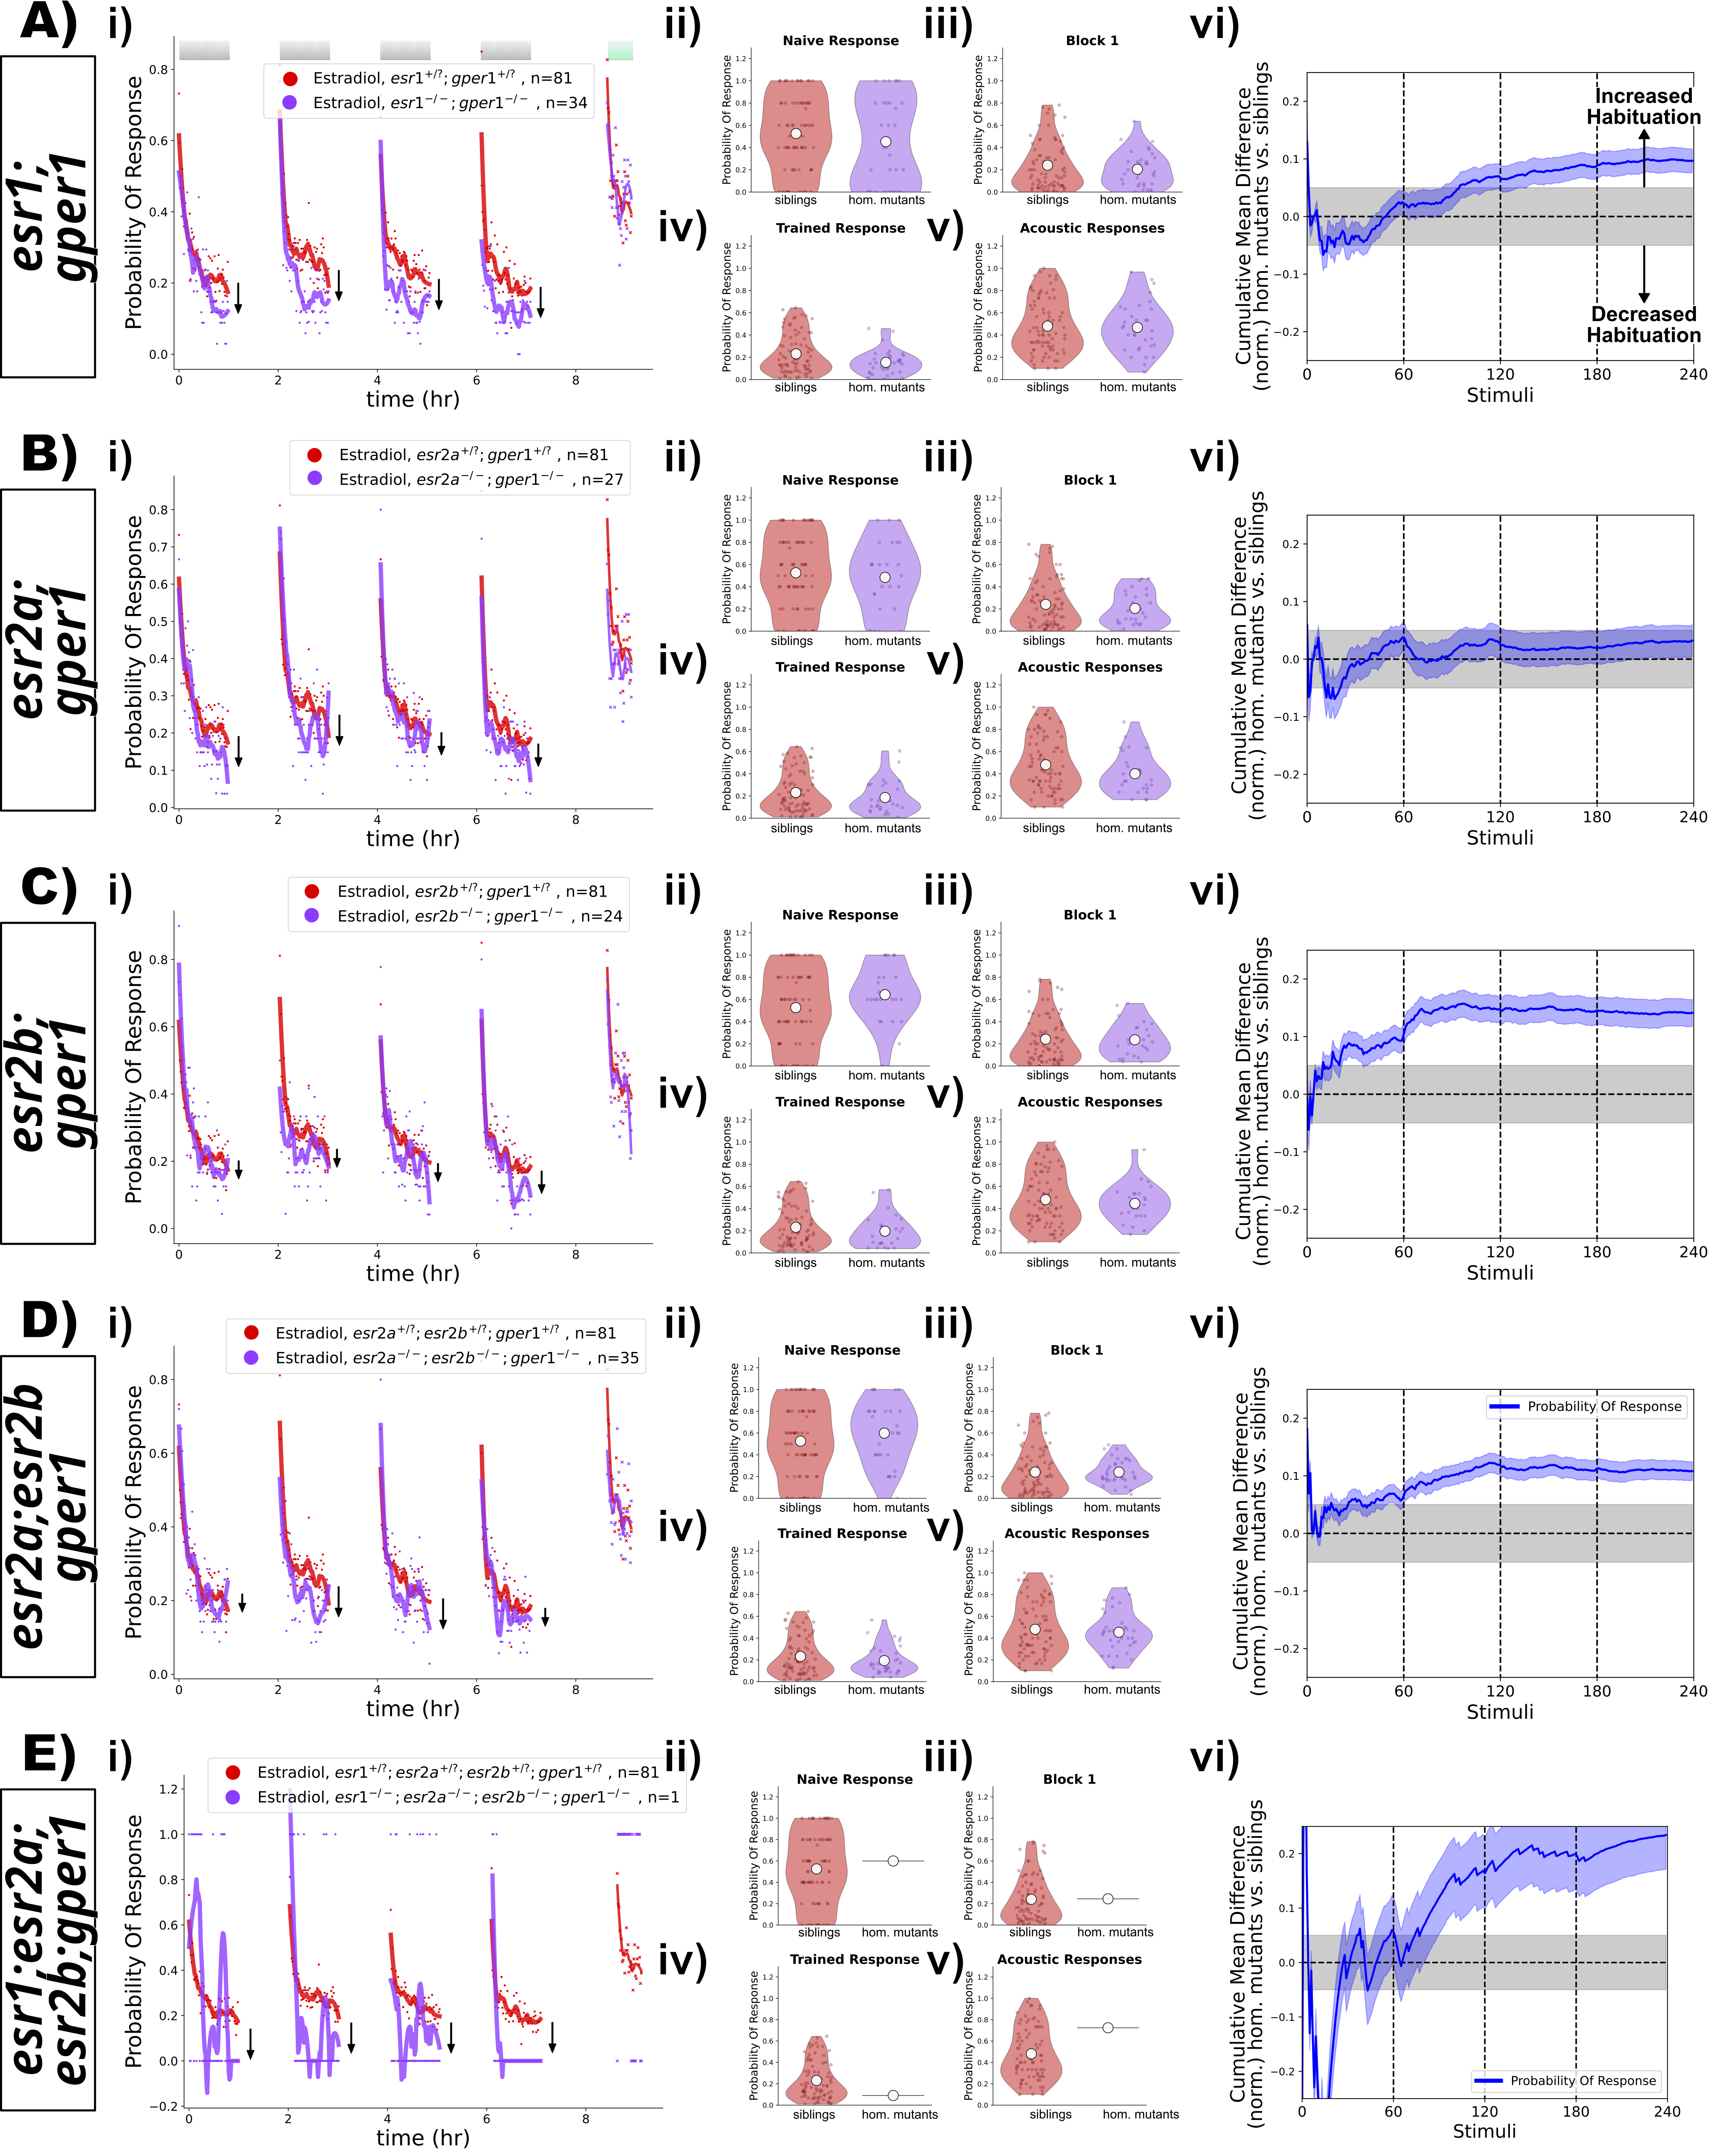
\includegraphics[width=0.95\linewidth]{figures/gper1andNuclearMutants.png}
\caption{ \textbf{Double and triple and quaruple mutant combinations of \emph{esr1}, \emph{esr2a}, \emph{esr2a}, and \emph{gper1} do not show habituation deficits after treatment with estradiol.}
\\ \textbf{A)} Homozygous \emph{esr1\textsuperscript{(-/-)}} mutants do not show impaired habituation relative to sibling het/wt controls. 
}
\label{fig:5}
\end{center}
\end{fullwidth}
\end{figure}

Finally, since it is formally possible that nuclear and membrane-initated estradiol-signaling could act in a redundant fashion, we analyzed combinations of double and triple mutants, but again failed to identify suppressions in habituation. 

\section{Funding}

This work was supported by funding from the ATIP-Avenir program of the CNRS and Inserm, a Fondation Fyssen research grant, and the IDEX-Impulsion initiative of the University of Lyon.

\section{Data Availability}

Software and analysis code is available here:  \href{https://github.com/owenrandlett/2025_HabEstrogen}{https://github.com/owenrandlett/2025\_HabEstrogen}. Datasets are available here: .

\bibliography{References_HabEstrogen}

\end{document}
